\documentclass[12pt,a4paper,oneside]{article}
\usepackage[colorlinks=true,unicode]{hyperref}
\usepackage[utf8]{inputenc}
\usepackage[czech]{babel}
\usepackage{graphicx}
\usepackage{pdfpages}
\textwidth 16cm \textheight 25cm
\topmargin -1.3cm 
\oddsidemargin 0cm
\usepackage{footnote}
\pagestyle{empty}
\begin{document}
\title{Softwarově definovaný přijímač SDRX01B nejen pro radioastronomii}
\author{Jakub Kákona, kaklik@mlab.cz }
\maketitle

\begin{abstract}
Cílem této konstrukce je vytvořit dostupný softwarově definovaný přijímač pro použití v radioastronomii. A nahradit tak původní čistě analogové konstrukce, jako RadioJOVE a další. Díky dosaženým parametrům je ale dobře použitelný i v jiných aplikacích, jako například přehledový přijímač pro radioamatéry nebo jako studijní pomůcka pro výuku VF techniky. 
\end{abstract}

\begin{figure} [htbp]
\begin{center}
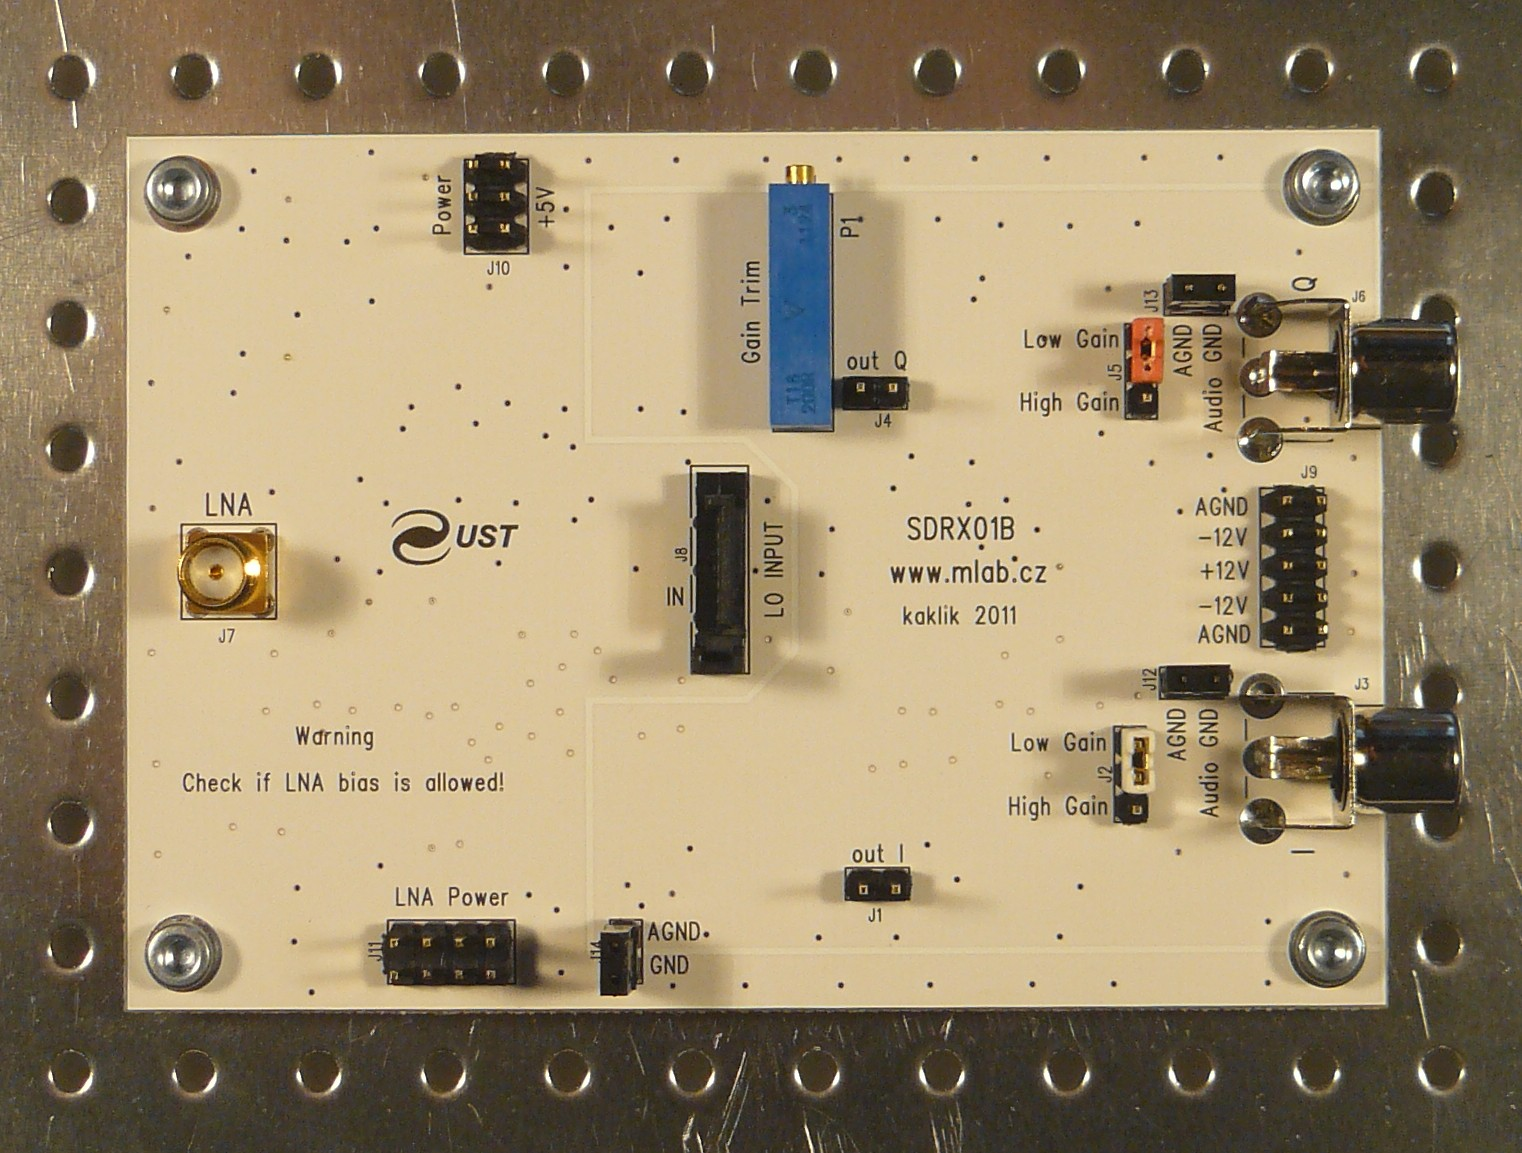
\includegraphics [width=80mm] {./img/SDRX01B_Top_Big.JPG} 
\end{center}
\end{figure}

\begin{figure} [b]

\includegraphics [width=25mm] {./img/SDRX01B_QRcode.png} 
\end{figure}

\newpage
\tableofcontents

\section{Technické parametry}
\begin{savenotes}
\begin{table}[htbp]
\begin{center}
\begin{tabular}{|c|c|p{5cm}|}
\hline
Parametr & Hodnota & \multicolumn{1}{|c|}{Poznámka} \\
\hline
Napájecí napětí analogové části & $\pm$12V \footnote{první kusy vyrobené do 1.8.2011 ale mohou mít osazené pouze 10V konenzátory 100uF} 100mA &  Typicky 30mA \\ \hline
Napájecí napětí digitální části & +5V &  300mA \\ \hline
Napájecí napětí LNA & do +20V &  max 500mA \\ \hline
Přijímaný frekvenční rozsah  & 0,5 - 200 MHz\footnote{Prakticky je omezen kvalitou vstupních spínačů směšovače} &  \\ \hline
Vstupní frekvenční rozsah LO  & 1 - 400 MHz \footnote{Digitální část je dimenzována do cca 1 GHz} & Limitem je LO  \\ \hline
IIP3  & $>$ 0 dB & Hodnota závisí na parametrech zvukové karty \\ \hline
MDS  & -120 dBm @ 1kHz BW & -117 dBm pro 3 dB nad šumem  \\ \hline
Potlačení zrcadlového příjmu   & $>$ 50 dB & Typicky 70dB \footnote{Hodnota závisí na přesnosti nastavení P1}\\ \hline
Zisk & 40-60dB & Lze částečně ovlivnit konfigurací NF zesílení\\ \hline
Šumové číslo  & $<$ 30dB & \\ \hline
\end{tabular}
\caption{Údaje uvedené v tabulce jsou platné pro příjem na frekvenci 150MHz.}
\label{Technicke_parametry}
\end{center}
\end{table}
\end{savenotes}

\newpage
\section{Popis konstrukce}

\subsection{Zapojení}
Zapojení přijímače vychází z původní konstrukce SDR přijímače DR2G \cite{DR2G}  který požívá CMOS součástky. Nyní je u přijímače změněný hlavně obvod vstupu pro lokální oscilátor a umožňuje tak používat přijímač na vyšších kmitočtech, neboť nedělí vstupní frekvenci 4mi, jako původní konstrukce ale pouze 2mi. To mimo jiné znamená, že nejvyšší pracovní kmitočet již není limitován vstupní logikou, ale analogovými spínači a v menší míře i převodníky LVPECL-CMOS těsně před spínači. Použitá diferenciální LVPECL logika navíc také umožňuje podstatně snížit vyzařování. Dále byly vyměněny analogové spínače ve směšovači. Ty nyní spínají trochu rychleji, ale hlavně mají lepší izolační parametry, což umožňuje lepší odstup signálu od šumu.

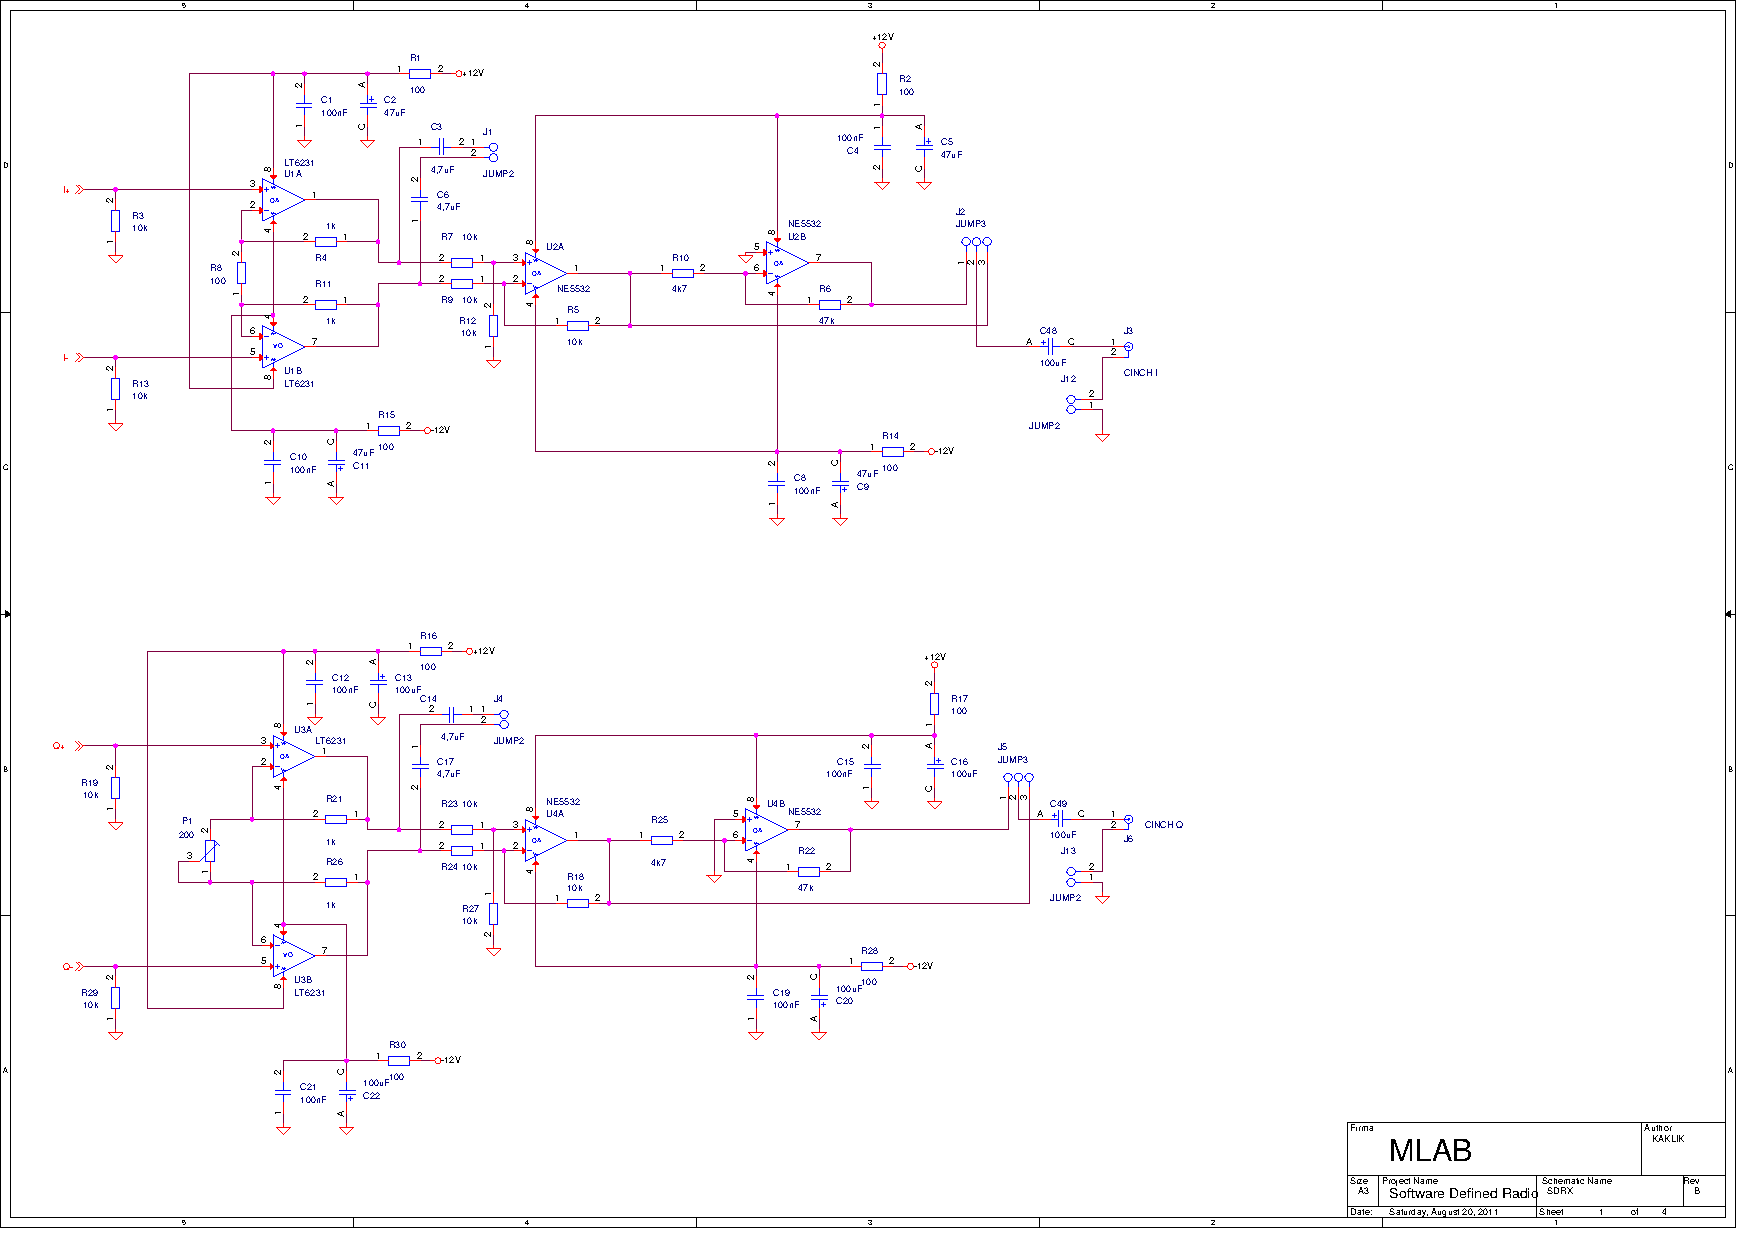
\includepdf[pages={1,2,3,4},landscape=true]{../../SCH/sdrx.pdf}

Další nezbytnou součástí přijímače je lokální oscilátor, který se připojuje k přijímači externě pomocí krátkého SATA kabelu. Jako LO lze použít modul CLKGEN01B osazený 570ABB000107DG. SATA kabel je vhodné volit co nejkratší kvůli minimalizaci zemní smyčky a vyzařování.


\subsection{Odrušení}
Pro správnou funkci přijímače je nutné řádné odrušení napájecích zdrojů. Vhodné je také omezit zemní smyčky a zem rozvádět pokud možno hvězdicově. Konstrukce obsahuje několik Jumperů, kterými je možné různými způsoby propojit země a eliminovat tak proudy tekoucí mezi nimi. Zvláště nežádoucí je proměnný proud tekoucí stíněním, například u výstupních CINCHů, Jumpery proto umožňují jejich odpojení od AGND přijímače. V tom případě se ale předpokládá propojení země ADC a AGND externím vedením, tak aby jím tekoucí proud neindukoval signál v analogových obvodech.
V některých případech (anténa uzemněna na hromosvod, nebo daleko od přijímače) se může vyskytnout problém se síťovým napájeným 50Hz indukovaným do svodu antény. Ten pak vytváří okolo nulové frekvence spektrogramu nežádoucí hrb, ten lze pak v takovém případě eliminovat oddělovacím transformátorem, na vstupu přijímače.     

Při provozu je také vhodné zabezpečit dostatečný útlum zpětně vyzařovaného útlumu ze směšovače, který by mohl rušit jiná zařízení a spoje. Na vstupu přijímače proto musí být zařazen izolační prvek, jako například LNA. 

\subsection{Mechanická konstrukce}

Mechanická konstrukce je řešena na dvouvrstvé desce s geometrií kompatibilní se základo\-vou deskou MLAB (Pro lepší odstínění přijímače je vhodné použít duralovou desku ALBASE). Dvouvrstvý plošný spoj je zvolen hlavně kvůli kvalitnímu odstínění okolního rušení horní měděnou vrstvou. To umožňuje přijímače instalovat i velmi blízko sebe případně i nad sebe avšak všechny konektory  kromě NF audio výstupu předpokládají přivedení kabelu kolmo na rovinu desky. SMA konektor je možné osadit i úhlový s přivede\-ním kabelu do boku, ale za cenu nepatrně vyššího útlumu úhlového konektoru. Při těsné montáži je potřeba počítat i s určitou teplotní stabilizací, neboť digitální část okolo spínaného směšovače má poměrně velký příkon a způsobuje zahřívání zhruba o 15$^\circ C$ nad okolní teplotu. Pokud je od přijímače vyžadována dlouhodobá stabilita je proto vhodné jej umístit do termostatovaného boxu společně s LO.

\section{Výroba}
Výrobu vlastní desky pro přijímač nemohu doporučit. Neboť domácí výroba je dvouvrstvého plošného spoje je náročná sama o sobě a tento motiv plošného spoje navíc obsahuje plošky pro komponenty s poměrně vysokou třídou přesnosti.

\subsection{Osazení}
Vlastní osazení přijímače předpokládá zvládnutí SMT technologie. Nejkomplikovanější část je letování analogových spínačů u kterých je nutné dát pozor na přehřátí a je tedy vhodné použít více tavidla. Následně je potřeba pod mikroskopem zkontrolovat kvalitu pájení (zkraty, nepřipojené nožičky).

\begin{figure} [h!tbp]
  \centering
  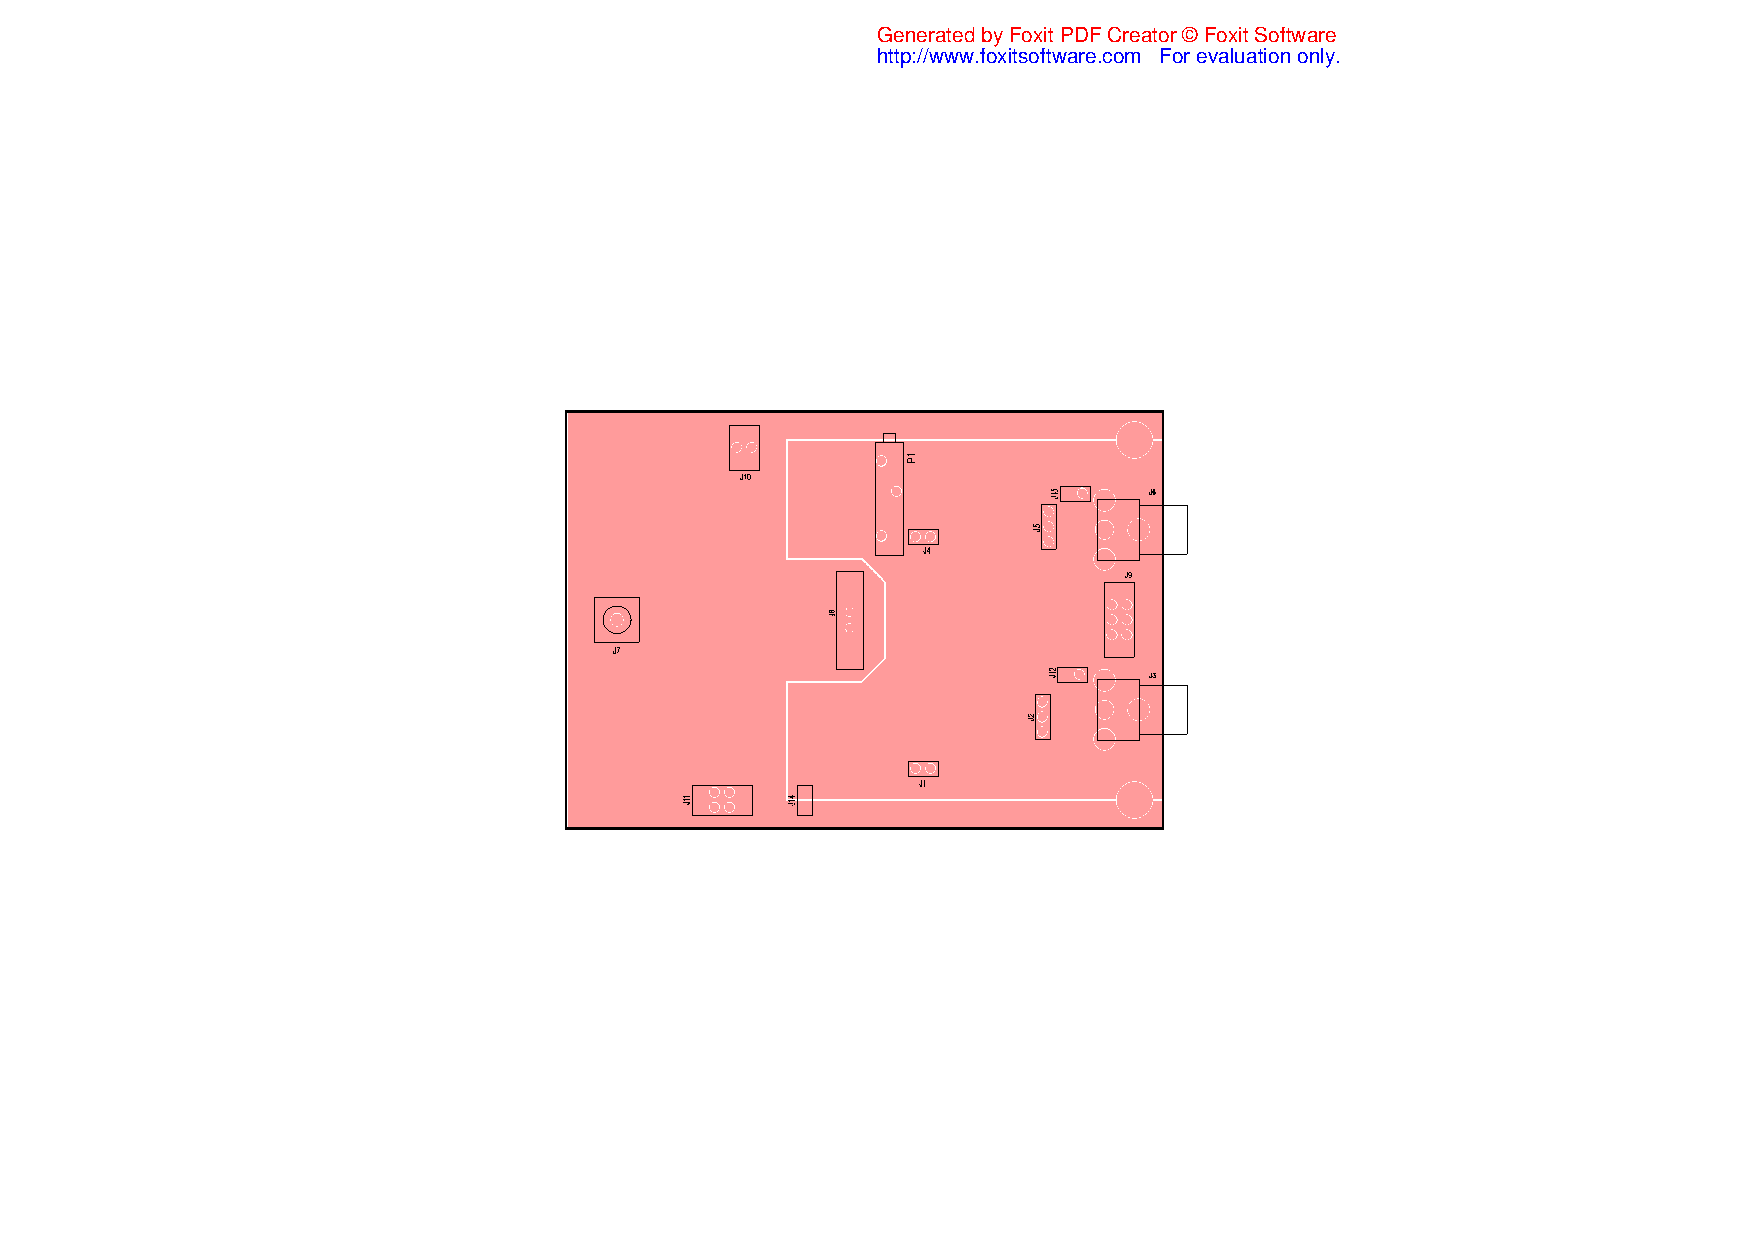
\includegraphics[trim = 9.5cm 6.5cm 8.5cm 6.5cm, clip, width=18.5cm]{../../CAM_DOC/O1.pdf}
  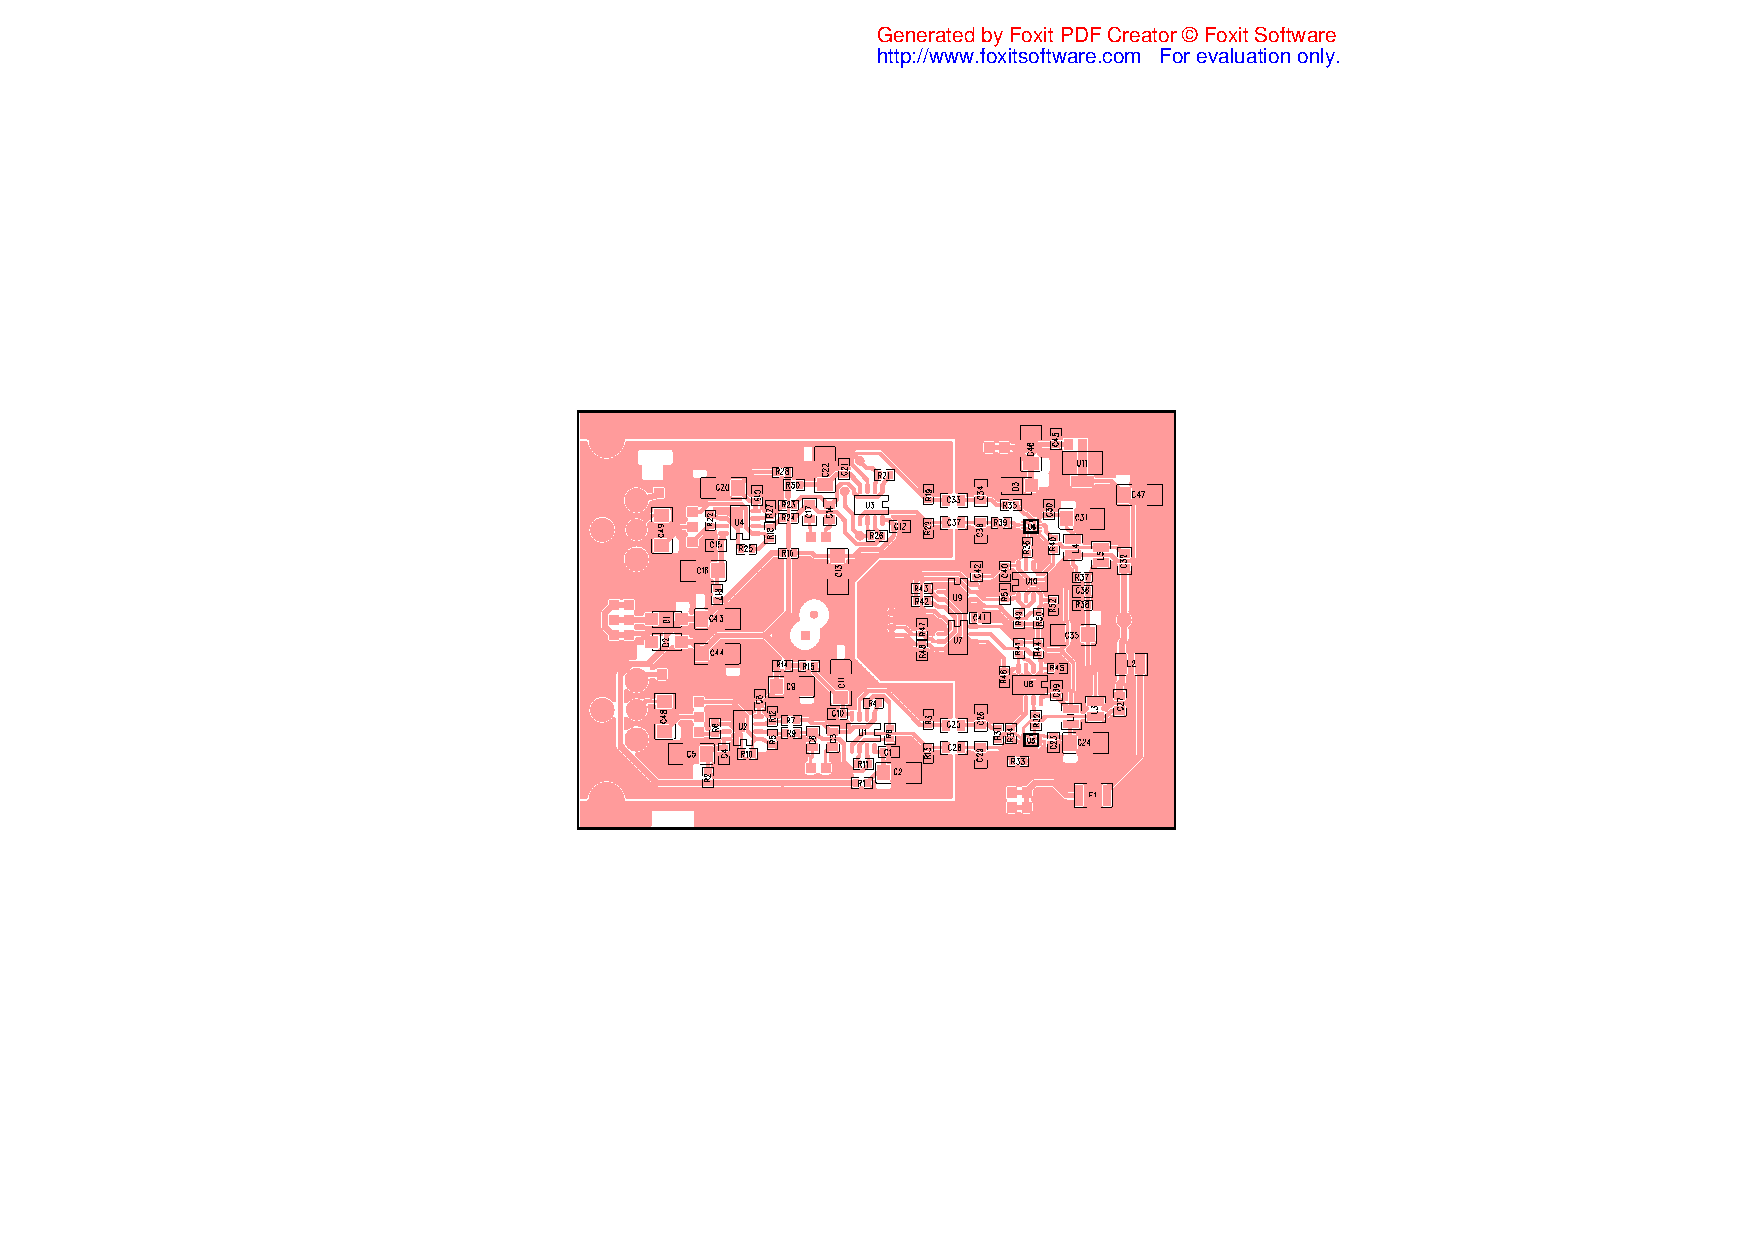
\includegraphics[trim = 9.5cm 6.5cm 9.0cm 6.5cm, clip, width=18cm]{../../CAM_DOC/O2.pdf}
  \caption{Osazovací plán horní a spodní strany plošného spoje}
  \label{fig:osazovaci_plan}
\end{figure}

\begin{table}[h!]
\begin{center}
\begin{tabular}{ |c|p{5cm}|c|c| }
\hline 
Počet & Označení & Typ  & Pouzdro  \\ 
\hline 
18	&	C1, C4, C8, C10, C12, C15, C19, C21, C23, C27, C30, C32, C36, C39, C40, C41, C42, C45	&	100nF	&	805	\\
17	&	C2, C5, C9, C11, C13, C16, C20, C22, C24, C31, C35, C43, C44, C46, C47, C48, C49	&	47uF	&	SMC	\\
4	&	C3, C6, C14, C17	&	4,7uF	&	805	\\
4	&	C25, C28, C33, C37	&	470nF	&	805	\\
4	&	C26, C29, C34, C38	&	22nF	&	805	\\
3	&	D1, D2, D3	&	M4	&	SMA	\\
1	&	F1	&	750mA	&		\\
5	&	J1, J4, J12, J13, J14	&	JUMP2	&		\\
2	&	J2,J5	&	JUMP3	&		\\
1	&	J3	&	CINCH I	&		\\
1	&	J6	&	CINCH Q	&		\\
1	&	J7	&	SMA6251A13G50	&		\\
1	&	J8	&	JUMP7	&		\\
1	&	J9	&	JUMP2X5	&		\\
1	&	J10	&	JUMP2X3	&		\\
1	&	J11	&	JUMP2X4	&		\\
5	&	L1, L2, L3, L4, L5	&	100uH	&		\\
1	&	P1	&	200	&	805	\\
13	&	R1, R2, R8, R14, R15, R16, R17, R28, R30, R32, R34, R36, R40	&	100	&	805	\\
12	&	R3, R5, R7, R9, R12, R13, R18, R19, R23, R24, R27, R29	&	10k 1\%	&	805	\\
4	&	R4,R11,R21,R26	&	1k 1\%	&	805	\\
2	&	R6,R22	&	47k 1\%	&	805	\\
2	&	R10,R25	&	4k7 1\%	&	805	\\
10	&	R31, R33, R35, R39, R45, R46, R47, R48, R51, R52	&	82	&	805	\\
2	&	R37,R38	&	330	&	805	\\
6	&	R41,R42,R43,R44,R49,R50	&	130	&	805	\\
2	&	U1,U3	&	LT6231	&	SO8	\\
2	&	U2,U4	&	NE5532	&	SO8	\\
2	&	U5,U6	&	NC7WB66	&		\\
2	&	U7,U9	&	MC100EP51	&	SO8	\\
2	&	U8,U10	&	SY100ELT23	&	SO8	\\
1	&	U11	&	LM1117MPX	&	SOT	\\
\hline 
\end{tabular}
\end{center}
\caption{Seznam součástek plošného spoje.}
\label{seznam_soucastek}
\end{table}

\subsection{Testování}
Testování přijímače spočívá v připojení na zdroje napájecího napětí s omezením proudu nastaveným na maximální hodnoty uvedené v tabulce \ref{Technicke_parametry}. Symetrický napájecí zdroj musí být dostatečně kvalitní a vyhlazený, aby nedocházelo k průniku rušení do analogové části. Je taktéž vhodné aby i symetrický zdroj měl proudové omezení. Pokud proudový odběr nepřekračuje stanovené limity. Můžeme připojit i lokální oscilátor. Pro testovací účely stačí použít modul CLKGEN01B pouze s připojeným napájením, tím dosáhneme přivedení jeho základní frekvence 10 MHz na vstupní děličku přijímače.  

Nyní můžeme osciloskopem zkontrolovat signál na vstupu analogových spínačů, kde by po připojení oscilátoru přes SATA kabel měl být měřitelný TTL signál. Se střídou 50 \% a frekvencí 5 MHz. Je potřeba změřit každý vstup spínače samostatně.  Pokud jsou analogové spínače v pořádku, lze pokračovat v ověření parametrů analogové části. To provedeme změřením napěťového offsetu na výstupním operačním zesilovači. Jeho hodnota by neměla být více než 1 V, měření je vhodné provádět osciloskopem, neboť tím lze detekovat i případné kmitání operačních zesilovačů. 

\subsection{Nastavení}

Následně je důležité nastavení shodných amplitud obou výstupních kanálů I a Q na stejnou hodnotu pomocí víceotáčkového trimru na horní straně desky. To lze udělat buď pomocí zvukové karty a minimalizace zrcadlových kmitočtů nějakého relativně silného AM vysílače. Nebo lze použít i metodu, kdy pomocí Jumperů, které slouží na výběr zesílení odpojíme jeden kanál (ten ve větvi s trimrem) a v softwaru si označíme aktuální úroveň signálu z antény. Pak analogicky kanál odpojíme připojíme naopak původně odpojený. Pomocí trimru pak nastavíme stejnou hodnotu signálu. Tento způsob je velmi jednoduchý a lze ho použít i za chodu, ale není příliš přesný. hodí se spíše na detekci poruchy (nefungující jeden z kanálů). 

Nejpřesnější metoda je použití signálového generátoru, který necháme vysílat do přijí\-ma\-če signálem cca -50dBm na požadovaném kmitočtu, kde potřebujeme přijímač zkalibrovat a trimrem nastavíme zrcadlový kmitočet ve spektrogramu na minimální hodnotu. Pokud nemáme signálový generátor lze využít například další přijímač SDRX01B s dalším lokálním oscilátorem. Který díky zpětnému vyzařování do antény umožní stejný postup.
Další jeměšjí potlačení zrcadlového kmitočtu lze provádět vhodným nastavením zesílení jednotlivých kanálů ADC a jejich fázovým posuvem. Většina programů pro SDR má proto možnost vyvážení amplitudy a fáze.  

\section{Programové vybavení}

Základním programovým vybavením jsou všechny softwary využívající zvukovou kartu v komplexním režimu (I/Q) pro vstup signálu. Tedy například programy jako Winrad, WinradHD, HDSDR či Spectrum Lab. Do kterých většinou stačí přidat knihovnu pro ovládání LO s Si570, nebo lokální oscilátor ovládat jiným softwarem.

\section{Důležité poznámky k používání}
\begin{itemize}
\item Vzhledem k použitému principu spínaného směšovače přijímač z principu poměrně silně vyzařuje zpět do antény. \textbf{Nesmí se proto využívat k poslechu chráněných pásem přímo bez izolačního členu na vstupu!} (izolačním členem je myšlen prvek, který zabezpečí dostatečný útlum signálu směřujícího do antény, obvykle jde o LNA, nebo izolační zesilovač)

\item Aktuální způsoby použití a poznatky uživatelů přijímače najdete na wiki stránce MLAB \cite{SDRX}.
\end{itemize}

\begin{thebibliography}{99}
\bibitem{DR2G}{Původní konstrukce přijímače DR2G} 
\href{http://yu1lm.qrpradio.com/SMT SDR RX DR2G-YU1LM.pdf}{http://yu1lm.qrpradio.com/SMT SDR RX DR2G-YU1LM.pdf}
\bibitem{SDRX}{MLAB wiki stránka přijímače SDRX01B} 
\href{http://wiki.mlab.cz/doku.php?id=cs:sdrx}{http://wiki.mlab.cz/doku.php?id=cs:sdrx}
\end{thebibliography}
\end{document}